% KubeEdgeInfer -- the simple 10-slide talk.
%
% Same content and the same measured numbers as kubeedgeinfer.tex, condensed to
% ten slides with larger type and fewer elements per slide. Compile with
% XeLaTeX or LuaLaTeX:
%
%     latexmk -xelatex kubeedgeinfer-simple.tex
%
% The code walkthrough (kubeedgeinfer-code.tex) stays a separate document.

\documentclass[aspectratio=169,11pt]{beamer}

\usepackage{booktabs}
\usepackage{array}
\usepackage{makecell}
\renewcommand\theadfont{\bfseries}
\usepackage{tikz}
\usepackage{pgfplots}
\pgfplotsset{compat=1.18}
\usetikzlibrary{arrows.meta,calc}

% ---------------------------------------------------------------- fonts
% Carlito and Caladea are the metric-compatible open equivalents of Calibri and
% Cambria -- the pairing the .pptx uses -- so this compiles the same anywhere.
% Have the real fonts? Swap Carlito -> Calibri and Caladea -> Cambria. No
% XeLaTeX? Replace this block with \usepackage{lmodern} and drop \headfont.
\usepackage{fontspec}
\setsansfont{Carlito}
\newfontfamily\headfont{Caladea}
\renewcommand{\familydefault}{\sfdefault}

% ---------------------------------------------------------------- palette
% One accent (teal) carries the deck; amber marks only the numbers that matter.
\definecolor{keink} {HTML}{1A1F2B}   % body text
\definecolor{kesoft}{HTML}{5A6377}   % secondary text
\definecolor{kemist}{HTML}{F2F4F8}   % the one background tint
\definecolor{keteal}{HTML}{1F8A80}
\definecolor{keamber}{HTML}{E07B39}
\definecolor{kepale}{HTML}{9AA2B0}

% ---------------------------------------------------------------- theme
\usetheme{default}
\setbeamertemplate{navigation symbols}{}
\setbeamercolor{normal text}{fg=keink,bg=white}
\setbeamercolor{structure}{fg=keteal}
\setbeamertemplate{frametitle}{%
  \vspace{0.6em}%
  {\headfont\LARGE\bfseries\color{keink}\insertframetitle}%
  \ifx\insertframesubtitle\empty\else
    \par\vspace{0.3em}{\small\color{kesoft}\insertframesubtitle}%
  \fi
  \par\vspace{0.4em}%
}
\setbeamertemplate{footline}{%
  \hfill{\tiny\color{kepale}\insertframenumber}\hspace{1.4em}\vspace{0.7em}}
\newcommand{\kefoot}[1]{\vfill\vspace{0.6em}{\scriptsize\itshape\color{kepale}#1}}

% ---------------------------------------------------------------- helpers
% The one repeated motif: a numbered teal circle beside a bold line.
\newcommand{\kedot}[2][keteal]{%
  \tikz[baseline=(n.base)]{\node[circle,fill=#1,text=white,inner sep=2pt,
    font=\small\bfseries,minimum size=1.9em] (n) {#2};}}
% #1 optional colour, #2 number, #3 heading, #4 body.
\newcommand{\kepoint}[4][keteal]{%
  \noindent\kedot[#1]{#2}\ \ {\large\bfseries\color{keink}#3}\par
  \vspace{0.15em}\hspace{2.5em}%
  \begin{minipage}{0.88\textwidth}{\small\color{kesoft}#4}\end{minipage}\par}
% One entry in the literature list: name, year, one-line summary.
\newcommand{\kepaper}[3]{%
  \noindent\textcolor{keteal}{$\bullet$}\ {\small\bfseries\color{keink}#1}\
  {\footnotesize\color{kesoft}(#2)}\par
  \hspace{1.1em}\begin{minipage}{\dimexpr\linewidth-1.1em\relax}%
    {\footnotesize\color{kesoft}#3}\end{minipage}\par\vspace{0.2em}}
% A soft tinted panel, used instead of bullet lists.
\newcommand{\kepanel}[2][kemist]{%
  \colorbox{#1}{\begin{minipage}{\dimexpr\linewidth-14pt\relax}
    \vspace{0.35em}#2\vspace{0.35em}\end{minipage}}}

\title{Sharing One Big AI Model Across Small Machines}
\author{}\date{}

\begin{document}

% =============================================================== 1. Title
\begin{frame}[plain]
  \vspace{1.6em}
  \noindent\tikz{\node[circle,fill=keteal,inner sep=3.4pt]{};}\ \
  {\small\bfseries\color{keteal}KubeEdgeInfer}\par\vspace{1.4em}
  {\headfont\fontsize{34}{42}\selectfont\bfseries\color{keink}
   Sharing One Big AI Model\\Across Small Machines}\par\vspace{0.7em}
  {\headfont\Large\itshape\color{keteal}and fixing the split while it runs}
  \par\vspace{1.2em}
  {\color{kesoft}Most systems decide how to cut the model once. We keep
   checking, and change the cut whenever the machines change.}
  \par\vspace{2.2em}
  {\small\color{kepale}Author:\qquad Institution:\qquad Date:}
\end{frame}

% =============================================================== 2. Introduction
\begin{frame}
  \frametitle{The machines keep changing}
  \begin{columns}[T]
  \begin{column}{0.63\textwidth}
    \vspace{0.4em}
    \kepoint{1}{A big model does not fit on one machine}{%
      So we cut it into blocks of layers and give one block to each machine.
      Where we cut is the most important choice we make.}
    \vspace{0.7em}
    \kepoint{2}{Small machines are not like data centres}{%
      Laptops and cheap GPU boxes get hot and slow down, their network speed
      wanders, and sometimes they switch off.}
    \vspace{0.5em}
    \kepoint[keamber]{3}{Other systems cut once and never look again}{%
      That cut is right at the start, and gets more and more wrong as the
      machines change.}
  \end{column}
  \begin{column}{0.33\textwidth}
    \vspace{0.4em}
    \kepanel{%
      {\bfseries\color{keamber}What that costs}\par\vspace{0.9em}
      {\headfont\fontsize{30}{34}\selectfont\bfseries\color{keink}2.4$\times$}\par
      {\small\color{kesoft}slower when one machine gets hot}\par\vspace{1.1em}
      {\headfont\fontsize{30}{34}\selectfont\bfseries\color{keink}4.3$\times$}\par
      {\small\color{kesoft}slower when the network slows too}}
  \end{column}
  \end{columns}
  \kefoot{Measured on slide 7, with 12 layers across 3 machines.}
\end{frame}

% =============================================================== 3. Literature
\begin{frame}[shrink=15]
  \frametitle{What others have done}
  \framesubtitle{Ten papers from 2024 and 2025. Full details on slide 10.}
  \begin{columns}[T]
  \begin{column}{0.47\textwidth}
    \kepaper{EdgeShard}{2024}{Picks where to cut with an exact solver. 50\% less delay.}
    \kepaper{Galaxy}{2024}{Splits work inside each layer instead of by layer.}
    \kepaper{Helix}{2025}{Chooses placement and routing together on mixed GPUs.}
    \kepaper{TPI-LLM}{2024}{Clever memory handling so 70B models fit in small RAM.}
    \kepaper{prima.cpp}{2025}{Runs 30--70B models on real home machines.}
  \end{column}
  \begin{column}{0.47\textwidth}
    \kepaper{Head-level splitting}{2025}{Cuts into very small pieces and moves them when memory is low.}
    \kepaper{Parallax}{2025}{Serves a model across volunteer machines, no central cluster.}
    \kepaper{Learned splitting}{2025}{Learns where to cut as the wireless signal changes.}
    \kepaper{Survey of the field}{2025}{Lists adapting to changing machines as an open problem.}
    \kepaper{Linux schedulers in eBPF}{2025}{Shows eBPF is now used to control, not only to watch.}
  \end{column}
  \end{columns}
  \vfill
  \kepanel{{\small\bfseries\color{keink}What they all have in common: they
    measure the machines before the run, and never measure again.}}
\end{frame}

% =============================================================== 4. Problem
\begin{frame}[shrink=10]
  \frametitle{The problem}
  \vspace{0.5em}
  \kepanel{%
    {\headfont\color{keink}We have $N$ model layers and $K$ machines of
     different speeds. While the model is answering, their speed, their network
     delay, and whether they are even alive all keep changing. Keep choosing a
     cut that makes the slowest machine as fast as possible --- and never
     restart anything to do it.}}
  \vspace{0.9em}\par
  {\small\bfseries\color{kesoft}That breaks into four jobs:}\par\vspace{0.5em}
  \begin{columns}[T]
  \begin{column}{0.47\textwidth}
    \kepoint{1}{Measure}{network delay and machine heat, cheaply, without
      changing the model code}
    \vspace{0.5em}
    \kepoint{3}{Act}{move layers between running machines without losing
      requests}
  \end{column}
  \begin{column}{0.47\textwidth}
    \kepoint{2}{Decide}{the best cut, fast enough to redo it often, without
      flip-flopping}
    \vspace{0.5em}
    \kepoint{4}{Recover}{notice a dead machine and share its layers among the
      rest}
  \end{column}
  \end{columns}
\end{frame}

% =============================================================== 5. Contributions
\begin{frame}
  \frametitle{What is new in our work}
  \vspace{0.6em}
  \kepoint{1}{We measure the network inside the kernel}{%
    Small eBPF programs read the round-trip time Linux already tracks for every
    connection. Others guess with timers, or measure only before the run.}
  \vspace{1.0em}
  \kepoint{2}{We never stop deciding}{%
    Watch, decide, act, recover --- every 2 seconds, for as long as the system
    runs. The cut is something we keep adjusting, not a setting we pick once.}
  \vspace{1.0em}
  \kepoint[keamber]{3}{We add brakes so it does not flip-flop}{%
    A new cut is applied only if it is at least 15\% better and 30 seconds have
    passed. The same brake handles heat, network and machine failure.}
  \vfill
  \kepanel[keink]{{\bfseries\color{white}We did not invent a new algorithm. We
    took the standard one and put it inside a loop that never stops
    measuring.}}
\end{frame}

% =============================================================== 6. Our system
\begin{frame}
  \frametitle{How our system works}
  \framesubtitle{The same four steps run over and over, every 2 seconds.}
  \vspace{0.4em}
  \centering
  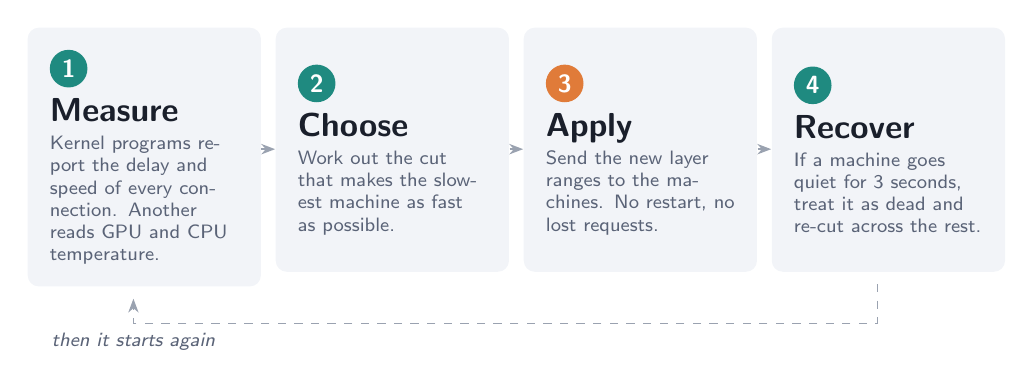
\begin{tikzpicture}[
      stepbox/.style={fill=kemist,rounded corners=4pt,text width=2.4cm,
                   align=left,inner sep=8pt,minimum height=3.1cm,
                   anchor=north west},
      font=\scriptsize]
    \node[stepbox] (a) at (0,0) {%
      \tikz{\node[circle,fill=keteal,text=white,inner sep=2pt,
            font=\small\bfseries,minimum size=1.8em]{1};}\\[0.4em]
      {\headfont\large\bfseries\color{keink}Measure}\\[0.3em]
      \color{kesoft}Kernel programs report the delay and speed of every
      connection. Another reads GPU and CPU temperature.};
    \node[stepbox] (b) at (3.15,0) {%
      \tikz{\node[circle,fill=keteal,text=white,inner sep=2pt,
            font=\small\bfseries,minimum size=1.8em]{2};}\\[0.4em]
      {\headfont\large\bfseries\color{keink}Choose}\\[0.3em]
      \color{kesoft}Work out the cut that makes the slowest machine as fast as
      possible.};
    \node[stepbox] (c) at (6.30,0) {%
      \tikz{\node[circle,fill=keamber,text=white,inner sep=2pt,
            font=\small\bfseries,minimum size=1.8em]{3};}\\[0.4em]
      {\headfont\large\bfseries\color{keink}Apply}\\[0.3em]
      \color{kesoft}Send the new layer ranges to the machines. No restart, no
      lost requests.};
    \node[stepbox] (d) at (9.45,0) {%
      \tikz{\node[circle,fill=keteal,text=white,inner sep=2pt,
            font=\small\bfseries,minimum size=1.8em]{4};}\\[0.4em]
      {\headfont\large\bfseries\color{keink}Recover}\\[0.3em]
      \color{kesoft}If a machine goes quiet for 3 seconds, treat it as dead and
      re-cut across the rest.};
    \foreach \x/\y in {a/b,b/c,c/d}
      \draw[-{Stealth[length=5pt]},kepale,thick]
        ($(\x.north east)+(0,-1.55cm)$) -- ($(\y.north west)+(0,-1.55cm)$);
    \draw[-{Stealth[length=5pt]},kepale,dashed]
      ($(d.south west)+(1.35cm,-0.15cm)$) -- ++(0,-0.5cm)
      -| ($(a.south west)+(1.35cm,-0.15cm)$)
      node[pos=0.5,below,font=\scriptsize\itshape,color=kesoft]
      {then it starts again};
  \end{tikzpicture}
  \par\vspace{0.9em}
  \kepanel{{\small\color{keink}Every plan carries a version number. Machines
    refuse messages from an old plan, and because they keep no state, the
    request is simply replayed.}}
\end{frame}

% =============================================================== 7. Results
\begin{frame}[shrink=12]
  \frametitle{Results}
  \framesubtitle{How slow the busiest machine gets. Lower is better.}
  \begin{columns}[T]
  \begin{column}{0.60\textwidth}
    \vspace{0.4em}
    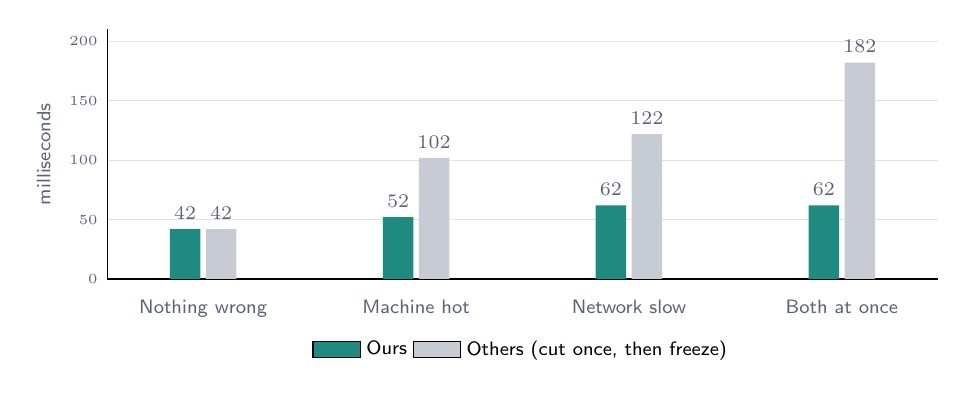
\begin{tikzpicture}
      \begin{axis}[
        width=\textwidth, height=4.75cm,
        ybar, bar width=11pt, enlarge x limits=0.15,
        ymin=0, ymax=210, ytick={0,50,100,150,200},
        ylabel={\scriptsize milliseconds}, ylabel style={color=kesoft},
        symbolic x coords={{Nothing wrong},{Machine hot},{Network slow},
                           {Both at once}},
        xtick=data, xticklabel style={font=\scriptsize,color=kesoft},
        yticklabel style={font=\tiny,color=kesoft},
        ymajorgrids, grid style={kepale!30},
        axis lines*=left, tick style={draw=none},
        nodes near coords, area legend,
        every node near coord/.append style={font=\scriptsize,color=kesoft},
        legend style={at={(0.5,-0.20)},anchor=north,legend columns=2,
                      draw=none,font=\scriptsize},
        ]
        \addplot[fill=keteal,draw=none] coordinates
          {({Nothing wrong},42) ({Machine hot},52)
           ({Network slow},62) ({Both at once},62)};
        \addplot[fill=kepale!55,draw=none] coordinates
          {({Nothing wrong},42) ({Machine hot},102)
           ({Network slow},122) ({Both at once},182)};
        \legend{Ours, Others (cut once{,} then freeze)}
      \end{axis}
    \end{tikzpicture}
  \end{column}
  \begin{column}{0.36\textwidth}
    \vspace{0.4em}
    \kepanel{{\headfont\fontsize{26}{30}\selectfont\bfseries\color{keteal}49\%}\par
      {\small\color{kesoft}better when a machine gets hot}}\par\vspace{0.45em}
    \kepanel{{\headfont\fontsize{26}{30}\selectfont\bfseries\color{keteal}66\%}\par
      {\small\color{kesoft}better when the network slows too}}\par\vspace{0.45em}
    \kepanel[keink]{{\headfont\large\bfseries\color{keamber}It keeps going}\par
      {\small\color{kepale}when a machine dies, the others take over. A fixed
       cut simply stops.}}
  \end{column}
  \end{columns}
  \kefoot{From \texttt{bench/dpsim}: 12 layers, 3 machines, one machine slowed
          to 0.4$\times$, 80\,ms network delay.}
\end{frame}

% =============================================================== 8. Comparison
\begin{frame}
  \frametitle{How we compare}
  \vspace{0.8em}
  \small
  \setcellgapes{5pt}\makegapedcells
  \begin{tabular}{@{}llllll@{}}
    \toprule
    & \thead[tl]{EdgeShard} & \thead[tl]{Galaxy} & \thead[tl]{Helix} &
      \thead[tl]{prima.cpp} & \thead[tl]{\color{keamber}Ours}\\
    \midrule
    Where its numbers come from & before the run & before the run &
      before the run & device specs &
      \makecell[tl]{\bfseries\color{keteal}live, from\\
                    \bfseries\color{keteal}the kernel}\\
    Re-cuts while running & no & no & only routing & no &
      \makecell[tl]{\bfseries\color{keteal}every 2 seconds}\\
    Reacts to a machine getting hot & no & no & no & no &
      \makecell[tl]{\bfseries\color{keteal}yes}\\
    Survives a machine dying & no & no & by copies & no &
      \makecell[tl]{\bfseries\color{keteal}yes, in 3 seconds}\\
    Changes without restarting & no & no & no & no &
      \makecell[tl]{\bfseries\color{keteal}yes}\\
    \bottomrule
  \end{tabular}
  \kefoot{We measure how slow the busiest machine gets. The other systems report
          different measurements, so the numbers are not directly comparable.}
\end{frame}

% =============================================================== 9. Conclusion
\begin{frame}
  \vspace{0.4em}
  \noindent\tikz{\node[circle,fill=keteal,inner sep=3pt]{};}\ \
  {\small\bfseries\color{keteal}Conclusion}\par\vspace{0.7em}
  {\headfont\fontsize{23}{30}\selectfont\bfseries\color{keink}
   Where to cut the model is a decision you should keep making, not one you
   make once.}\par\vspace{0.9em}
  \kepoint{1}{Working out the best cut is cheap}{%
    It takes microseconds, so there is no reason to do it only once.}
  \vspace{0.45em}
  \kepoint{2}{The brakes are what make it usable}{%
    One ``must be clearly better'' rule and one ``wait a bit'' rule handle heat,
    slow networks and dead machines the same way.}
  \vspace{0.45em}
  \kepoint{3}{Measuring in the kernel is free}{%
    eBPF sees what really went over the network, not what the program thinks it
    sent.}
  \kefoot{Next: support a Llama-size model, and calibrate the estimate so it
          predicts real speed, not only the right ranking.}
\end{frame}

% =============================================================== 10. References
\begin{frame}
  \frametitle{References}
  \scriptsize\color{kesoft}
  \begin{enumerate}\itemsep0.08em
    \item EdgeShard: Efficient LLM Inference via Collaborative Edge Computing.
      M.~Zhang, J.~Cao, X.~Shen, Z.~Cui. \emph{IEEE Internet of Things Journal},
      2024. arXiv:2405.14371.
    \item Galaxy: A Resource-Efficient Collaborative Edge AI System for In-situ
      Transformer Inference. \emph{IEEE INFOCOM}, 2024. arXiv:2405.17245.
    \item Helix: Serving Large Language Models over Heterogeneous GPUs and
      Network via Max-Flow. \emph{ACM ASPLOS}, 2025. arXiv:2406.01566.
    \item TPI-LLM: Serving 70B-scale LLMs Efficiently on Low-resource Edge
      Devices. 2024. arXiv:2410.00531.
    \item Prima.cpp: Fast 30--70B LLM Inference on Heterogeneous and
      Low-Resource Home Clusters. 2025. arXiv:2504.08791.
    \item Large Language Model Partitioning for Low-Latency Inference at the
      Edge. 2025. arXiv:2505.02533.
    \item Parallax: Efficient LLM Inference Service over Decentralized
      Environment. 2025. arXiv:2509.26182.
    \item Adaptive layer splitting for wireless large language model inference
      in edge computing. \emph{FITEE}, Springer, 2025.
      doi:10.1631/FITEE.2400468.
    \item Distributed LLMs and Multimodal Large Language Models: A Survey.
      2025. arXiv:2503.16585.
    \item Towards Agentic OS: An LLM Agent Framework for Linux Schedulers.
      2025. arXiv:2509.01245.
  \end{enumerate}
  \kefoot{Tools used: cilium/ebpf, Kubernetes, NVIDIA NVML, k3s, Hugging Face
          Transformers.}
\end{frame}

\end{document}
